%!TEX root=../../main.tex

\subsection{Breadth-first search}
In these figures, Galois with 96 threads is shown. Again, we show the impact of Galois' thread count in \autoref{sec:galois_speedup}.
\begin{figure*}
	\begin{subfigure}{0.3\textwidth}
		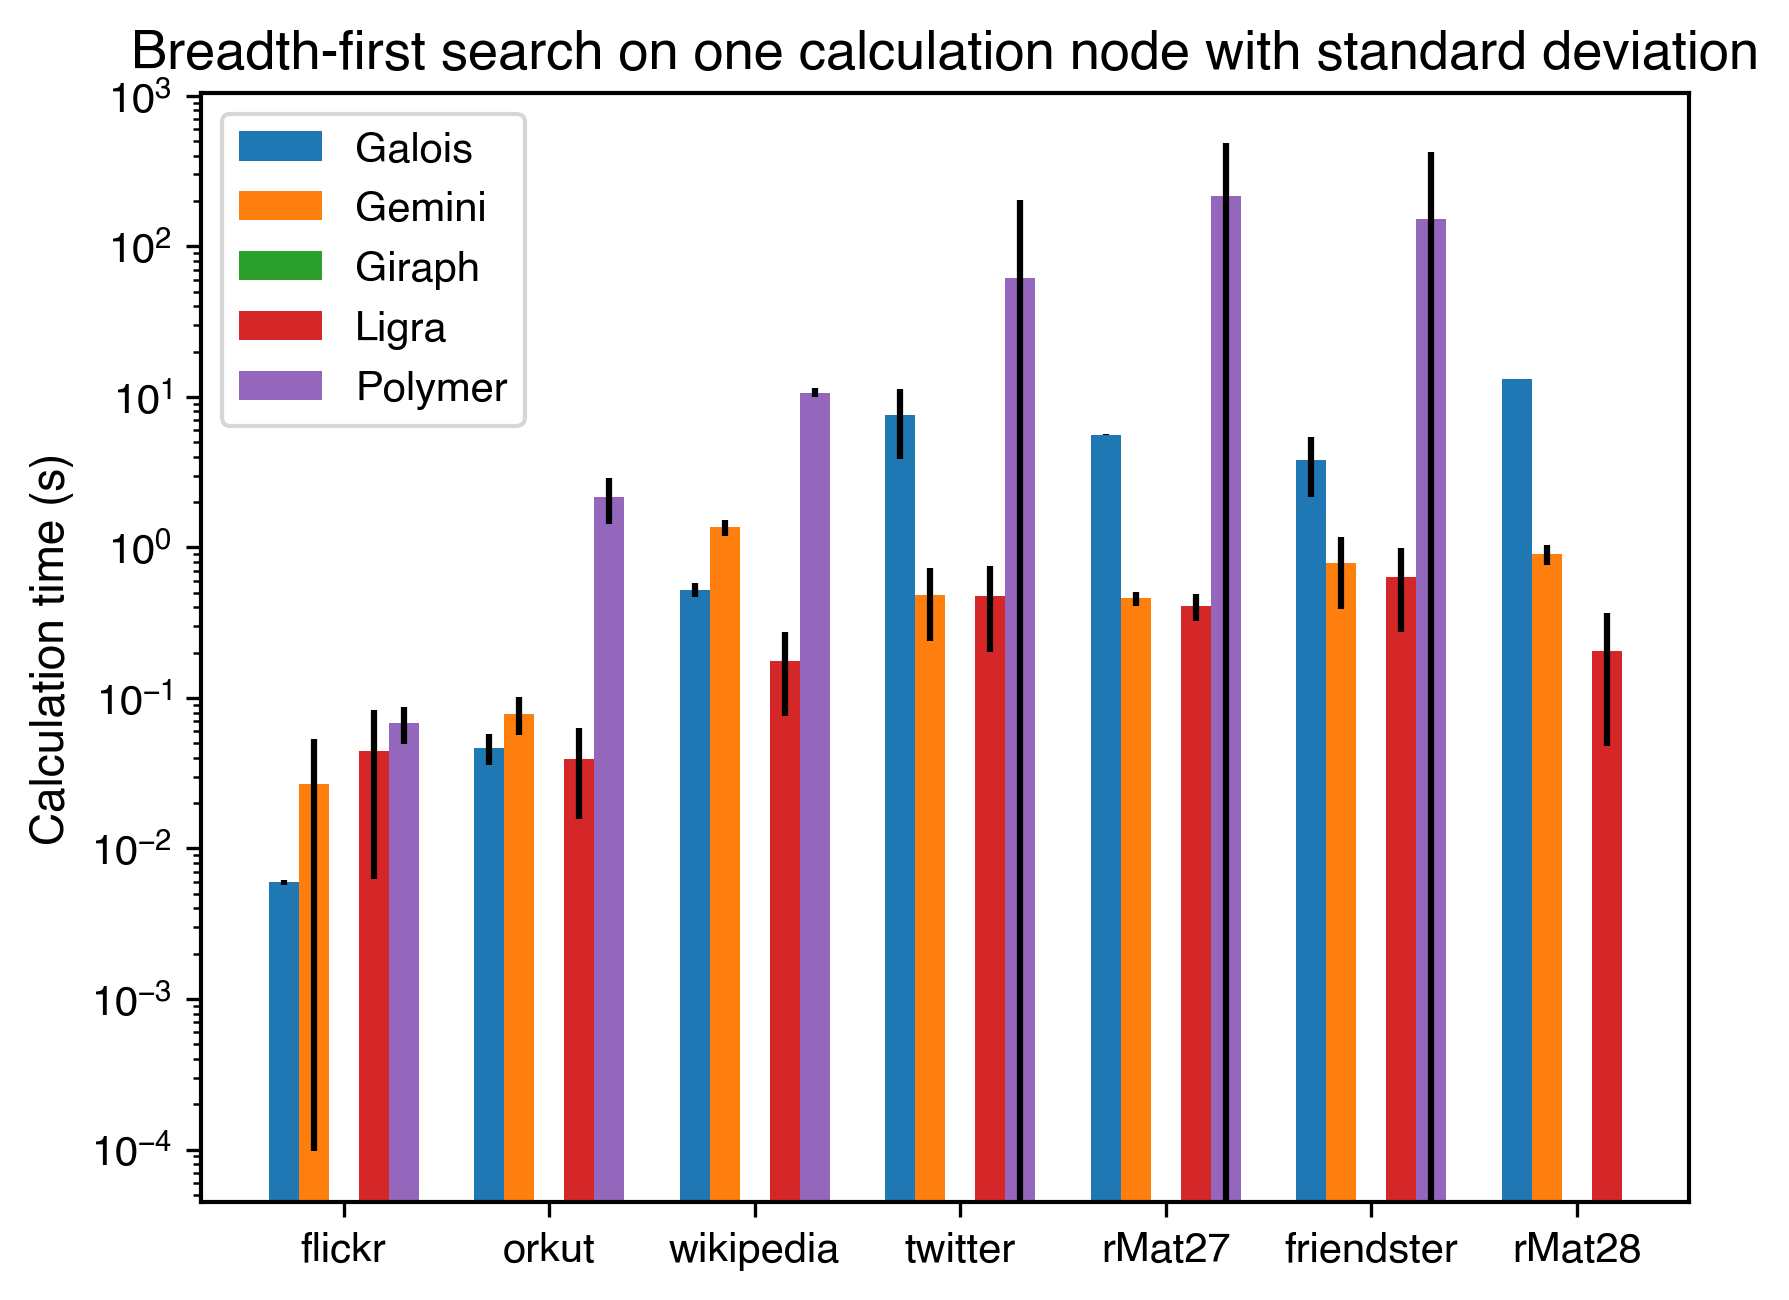
\includegraphics[width=\linewidth]{../../plots/singleNodeBFS_calcTime.png}
		\caption{Calculation times for BFS on a single node}
		\label{fig:singleNodeBFS_calc}
	\end{subfigure}
	\hfil
	\begin{subfigure}{0.3\textwidth}
		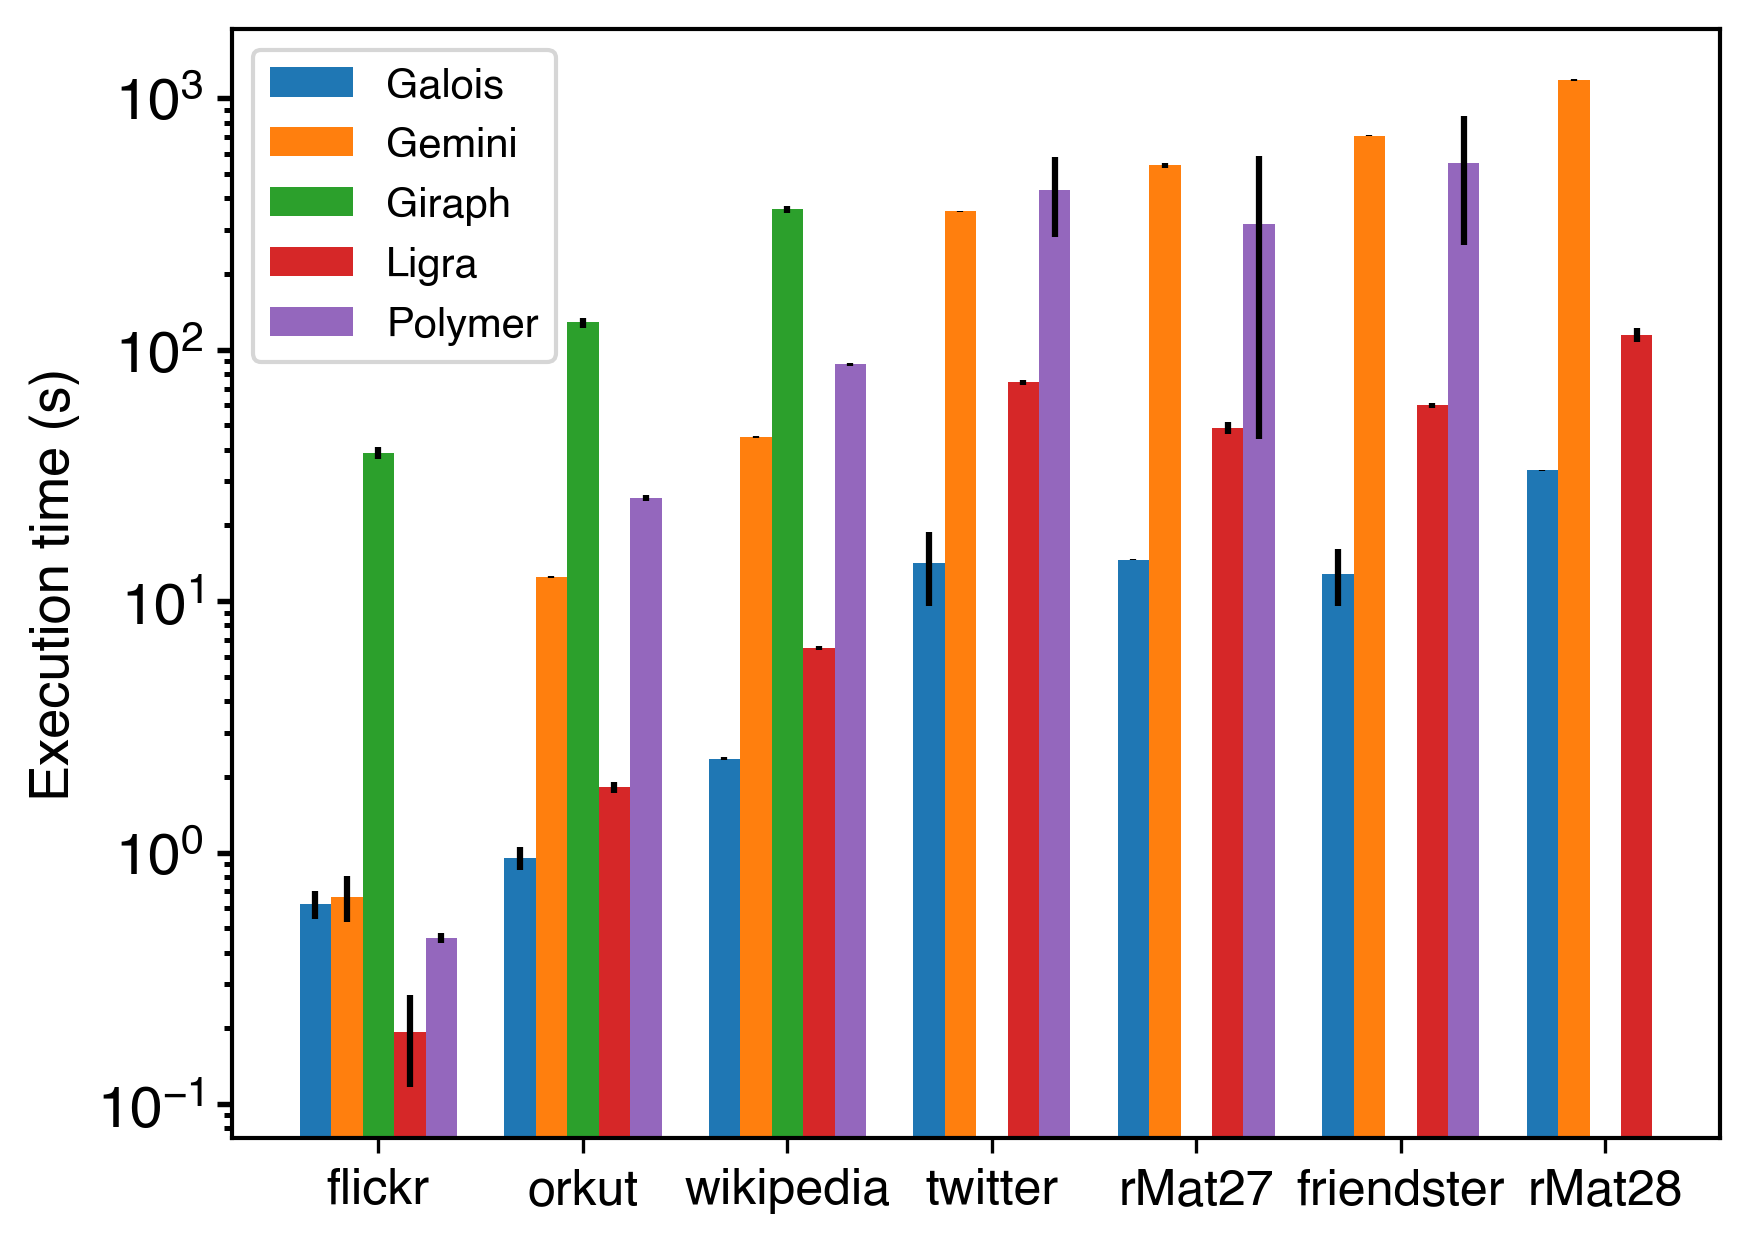
\includegraphics[width=\linewidth]{../../plots/singleNodeBFS_execTime.png}
		\caption{Execution times for BFS on a single node}
		\label{fig:singleNodeBFS_exec}
	\end{subfigure}
	\hfil
	\begin{subfigure}{0.3\textwidth}
		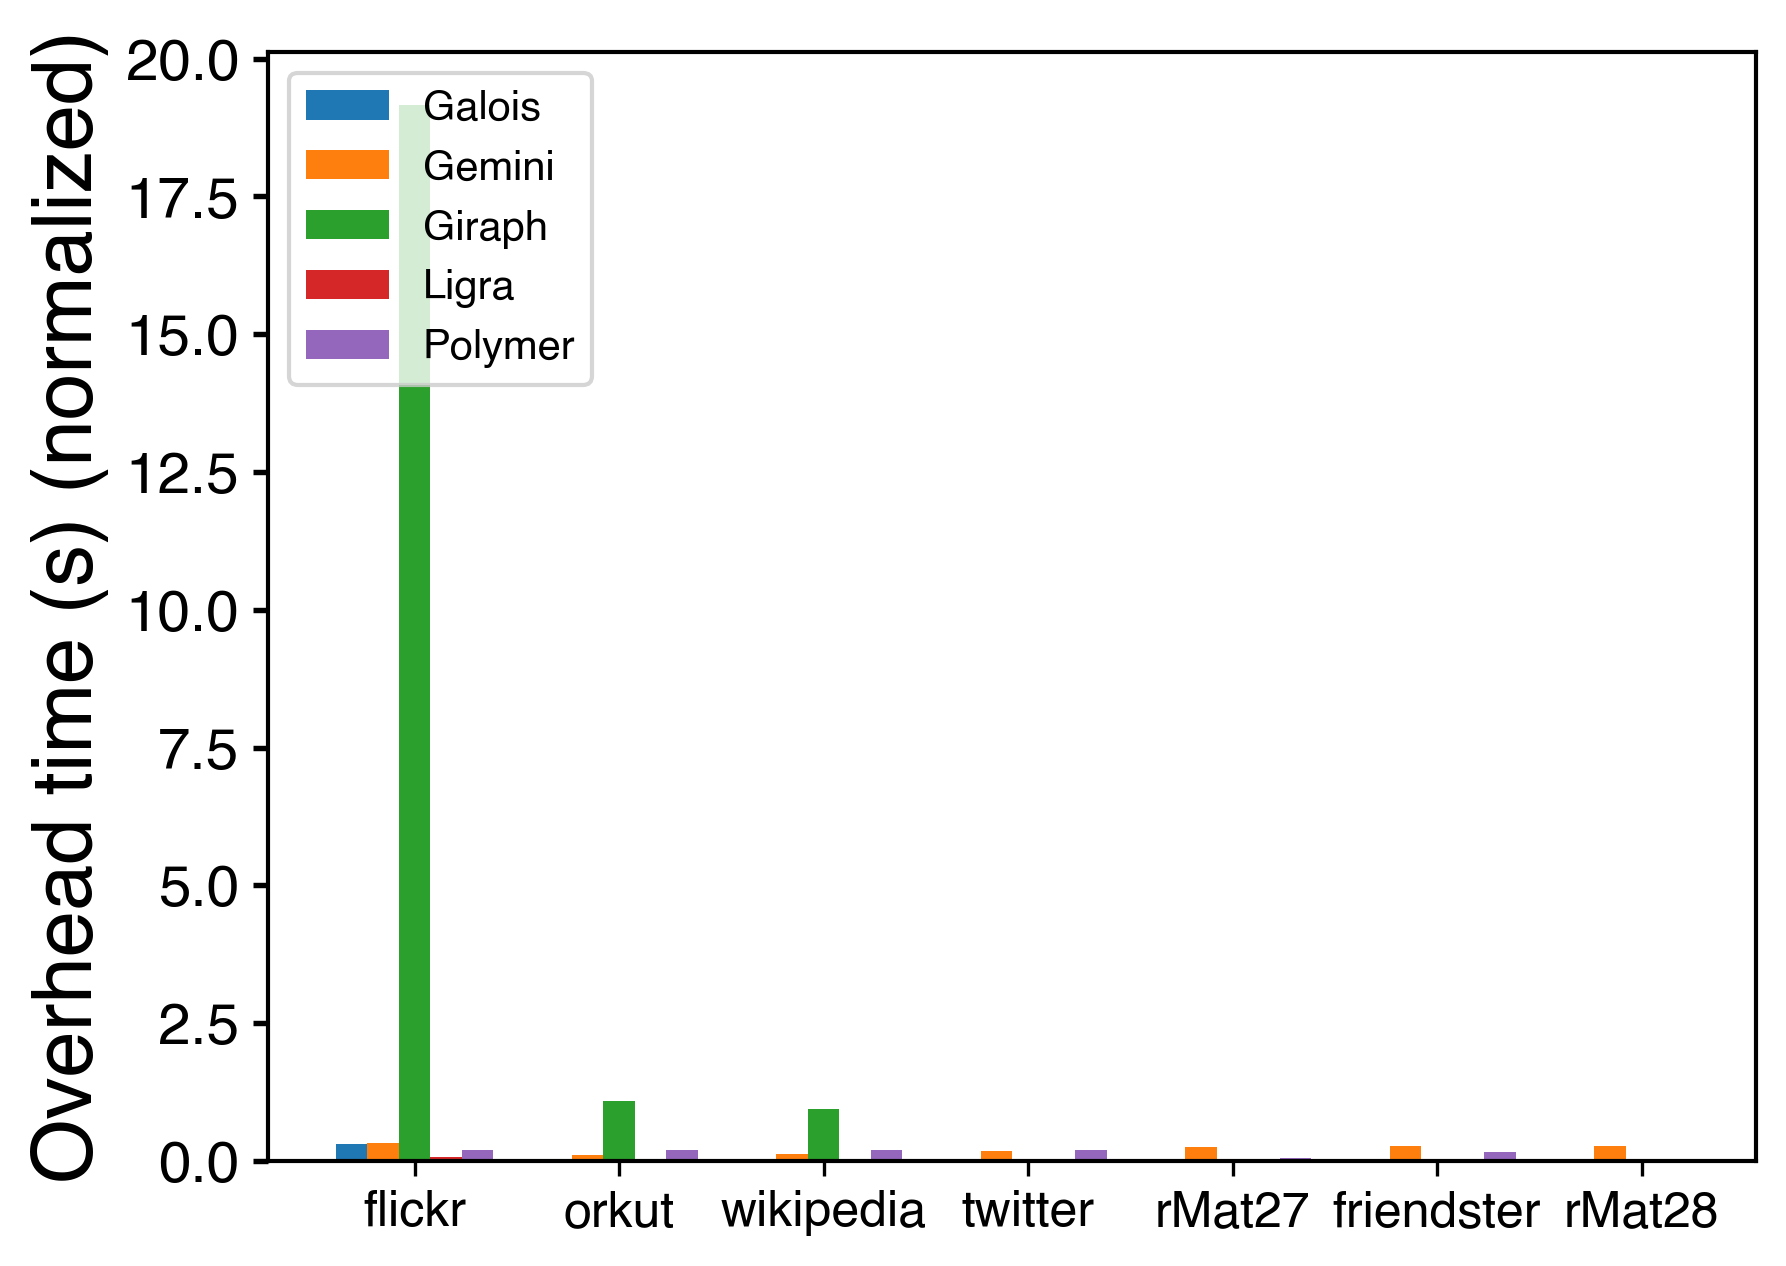
\includegraphics[width=\linewidth]{../../plots/singleNodeBFS_overheadTimeNormalized.png}
		\caption{Overhead time normalized by the graph size in million edges}
		\label{fig:singleNodeBFS_overheadNormalized}
	\end{subfigure}
	
	\caption{Average times on a single computation node, black bars represent one standard deviation in our testing}
\end{figure*}




\begin{figure*}
	\begin{subfigure}{0.3\textwidth}
		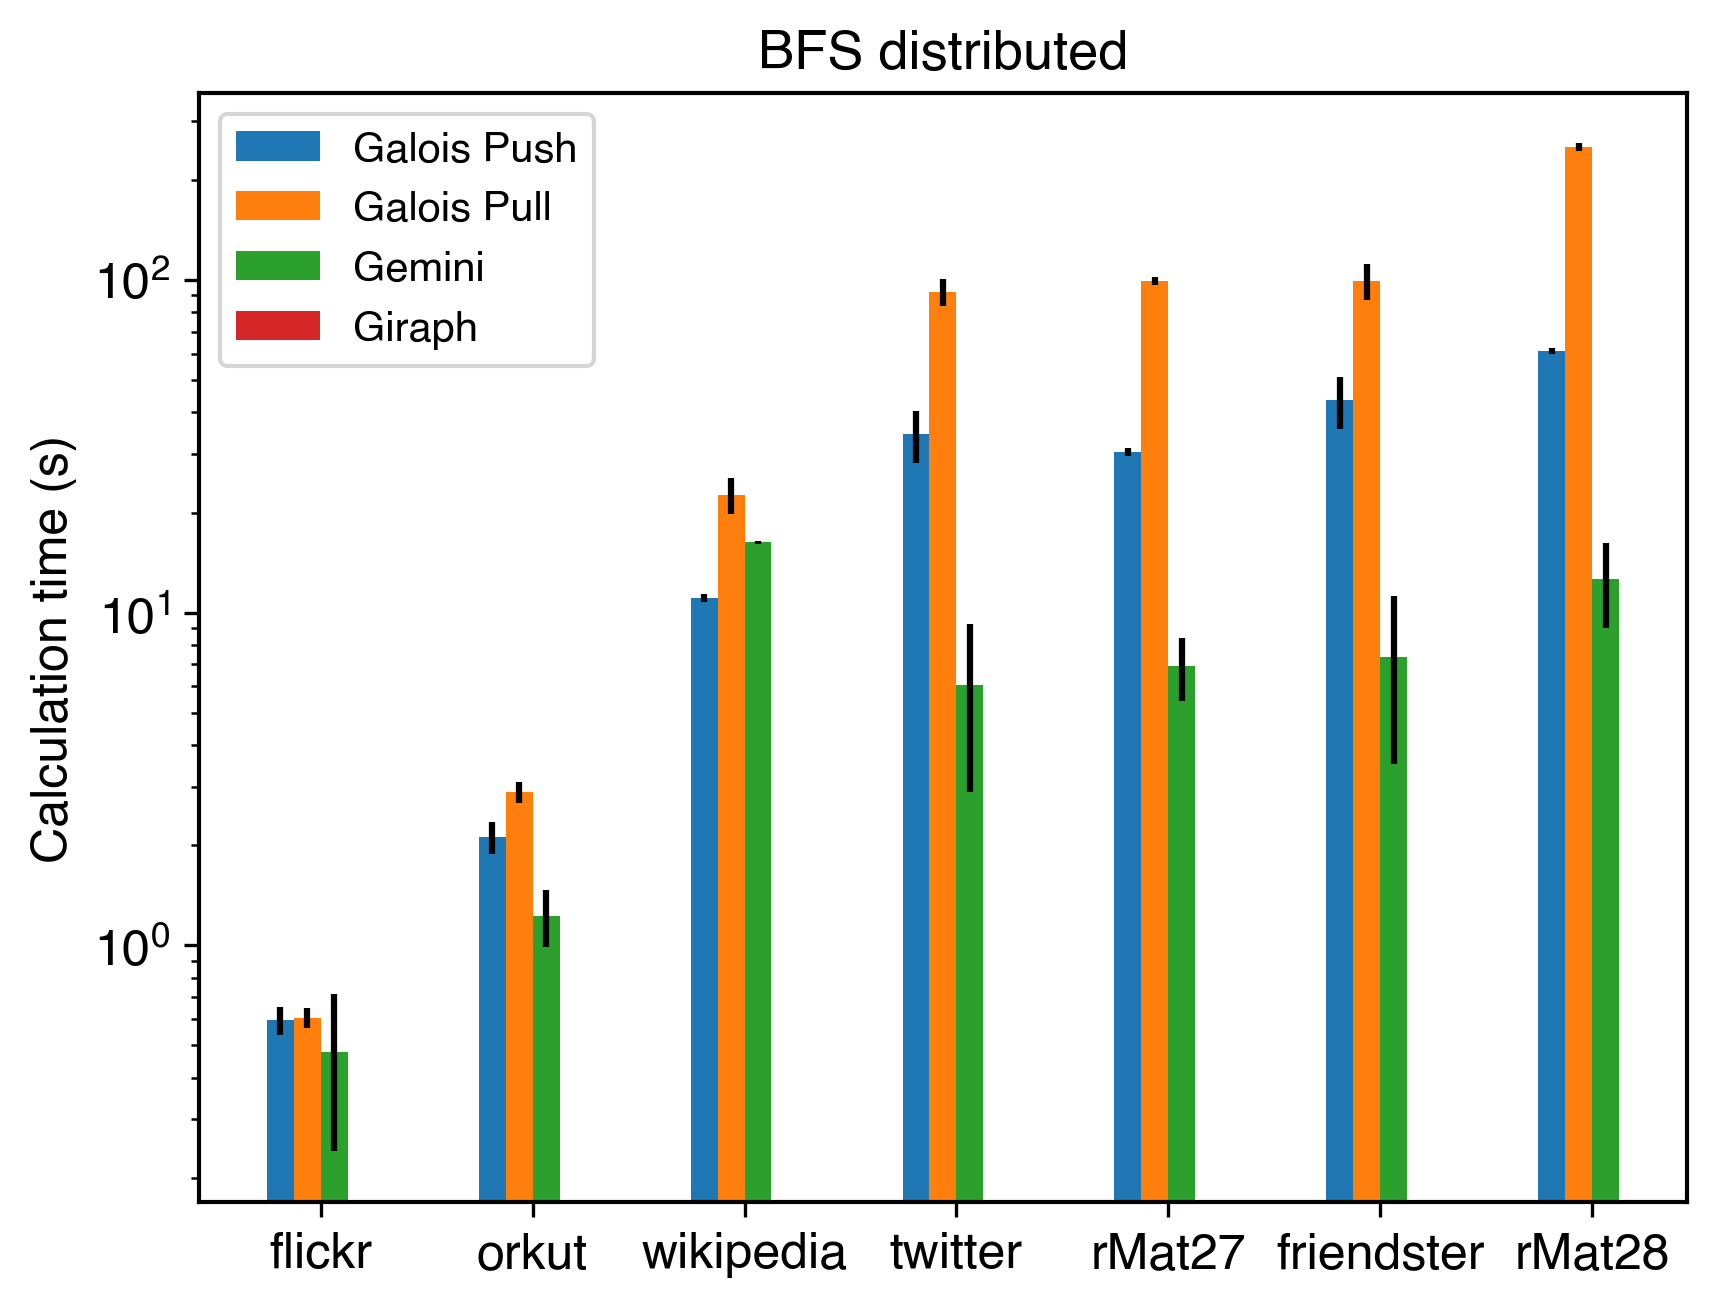
\includegraphics[width=\linewidth]{../../plots/distributedBFS_calcTime.png}
		\caption{Calculation times for distributed BFS}
		\label{fig:distributedBFS_calc}
	\end{subfigure}
	\hfil
	\begin{subfigure}{0.3\textwidth}
		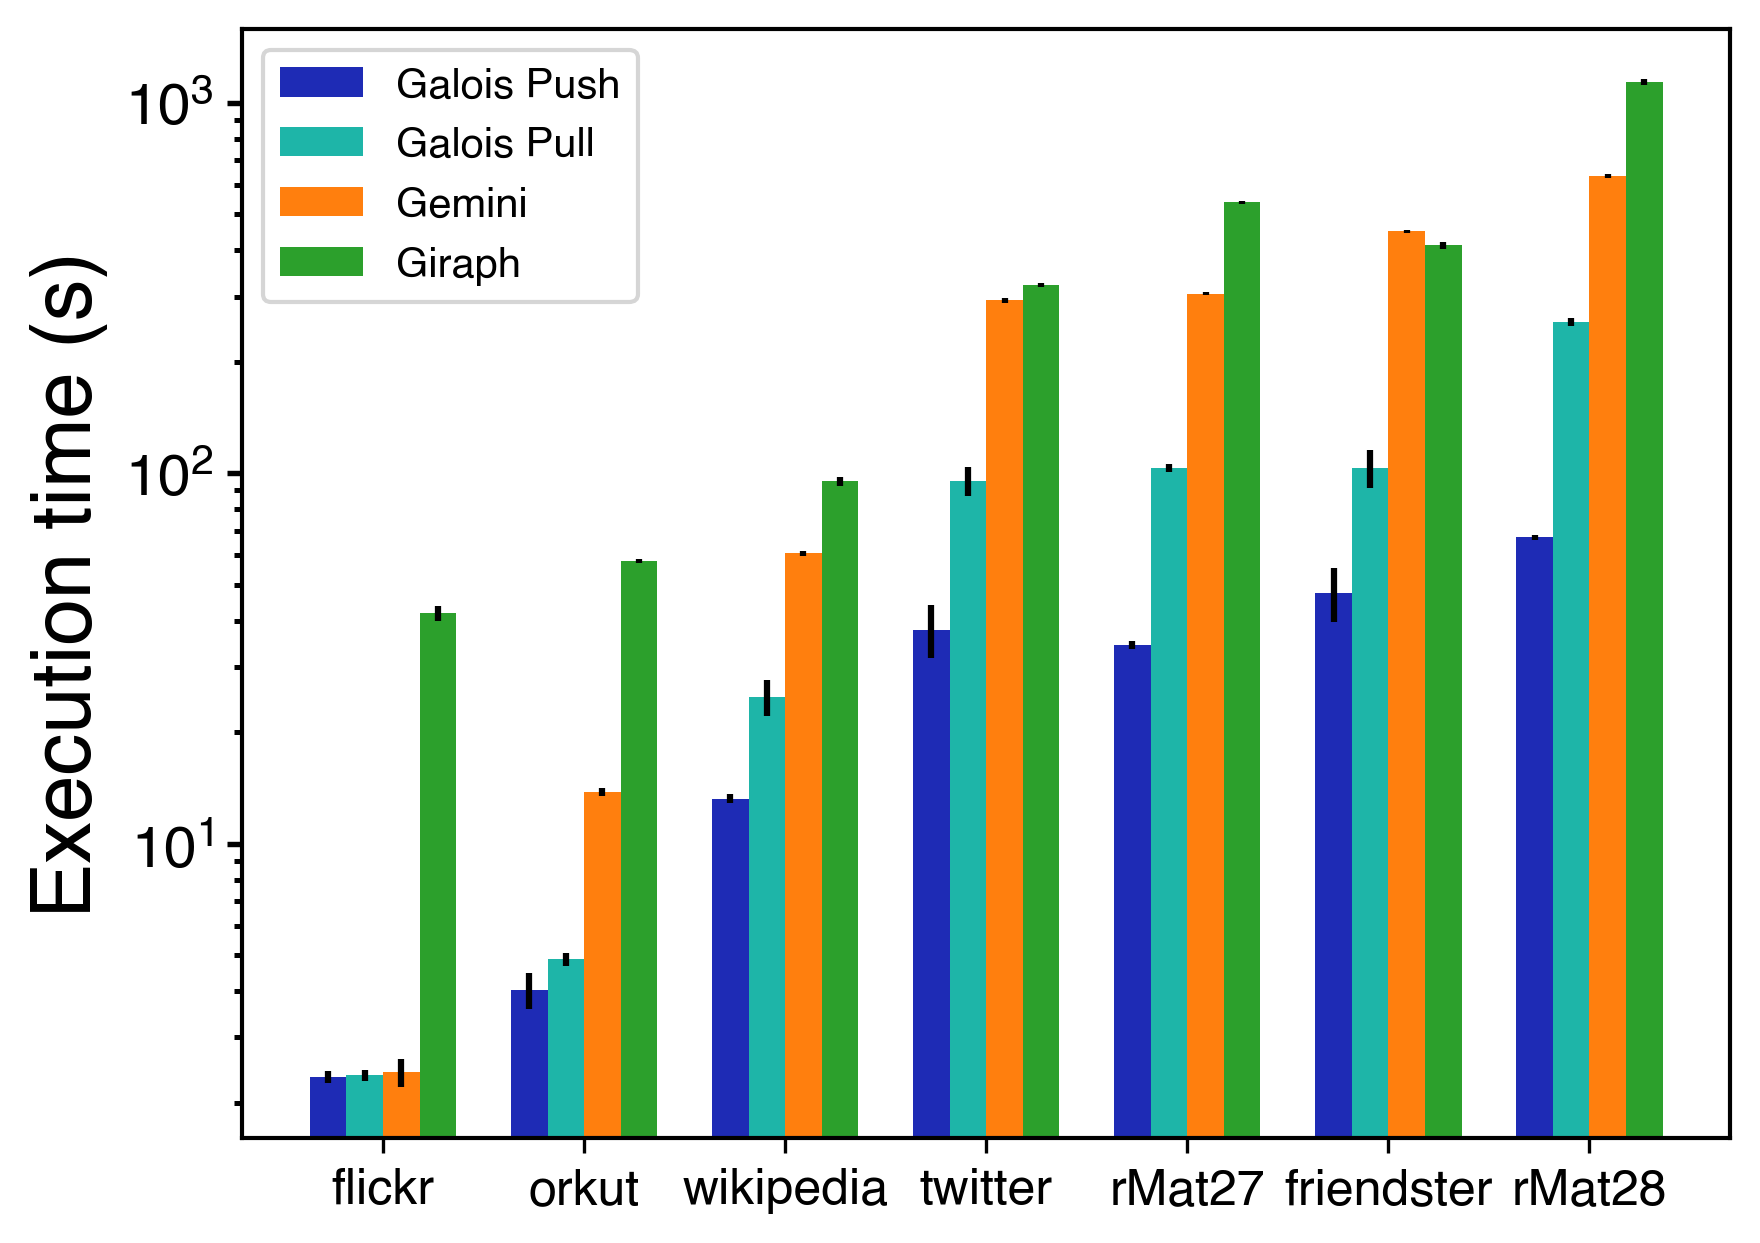
\includegraphics[width=\linewidth]{../../plots/distributedBFS_execTime.png}
		\caption{Execution times for distributed BFS}
		\label{fig:distributedBFS_exec}
	\end{subfigure}
	\hfil
	\begin{subfigure}{0.3\textwidth}
		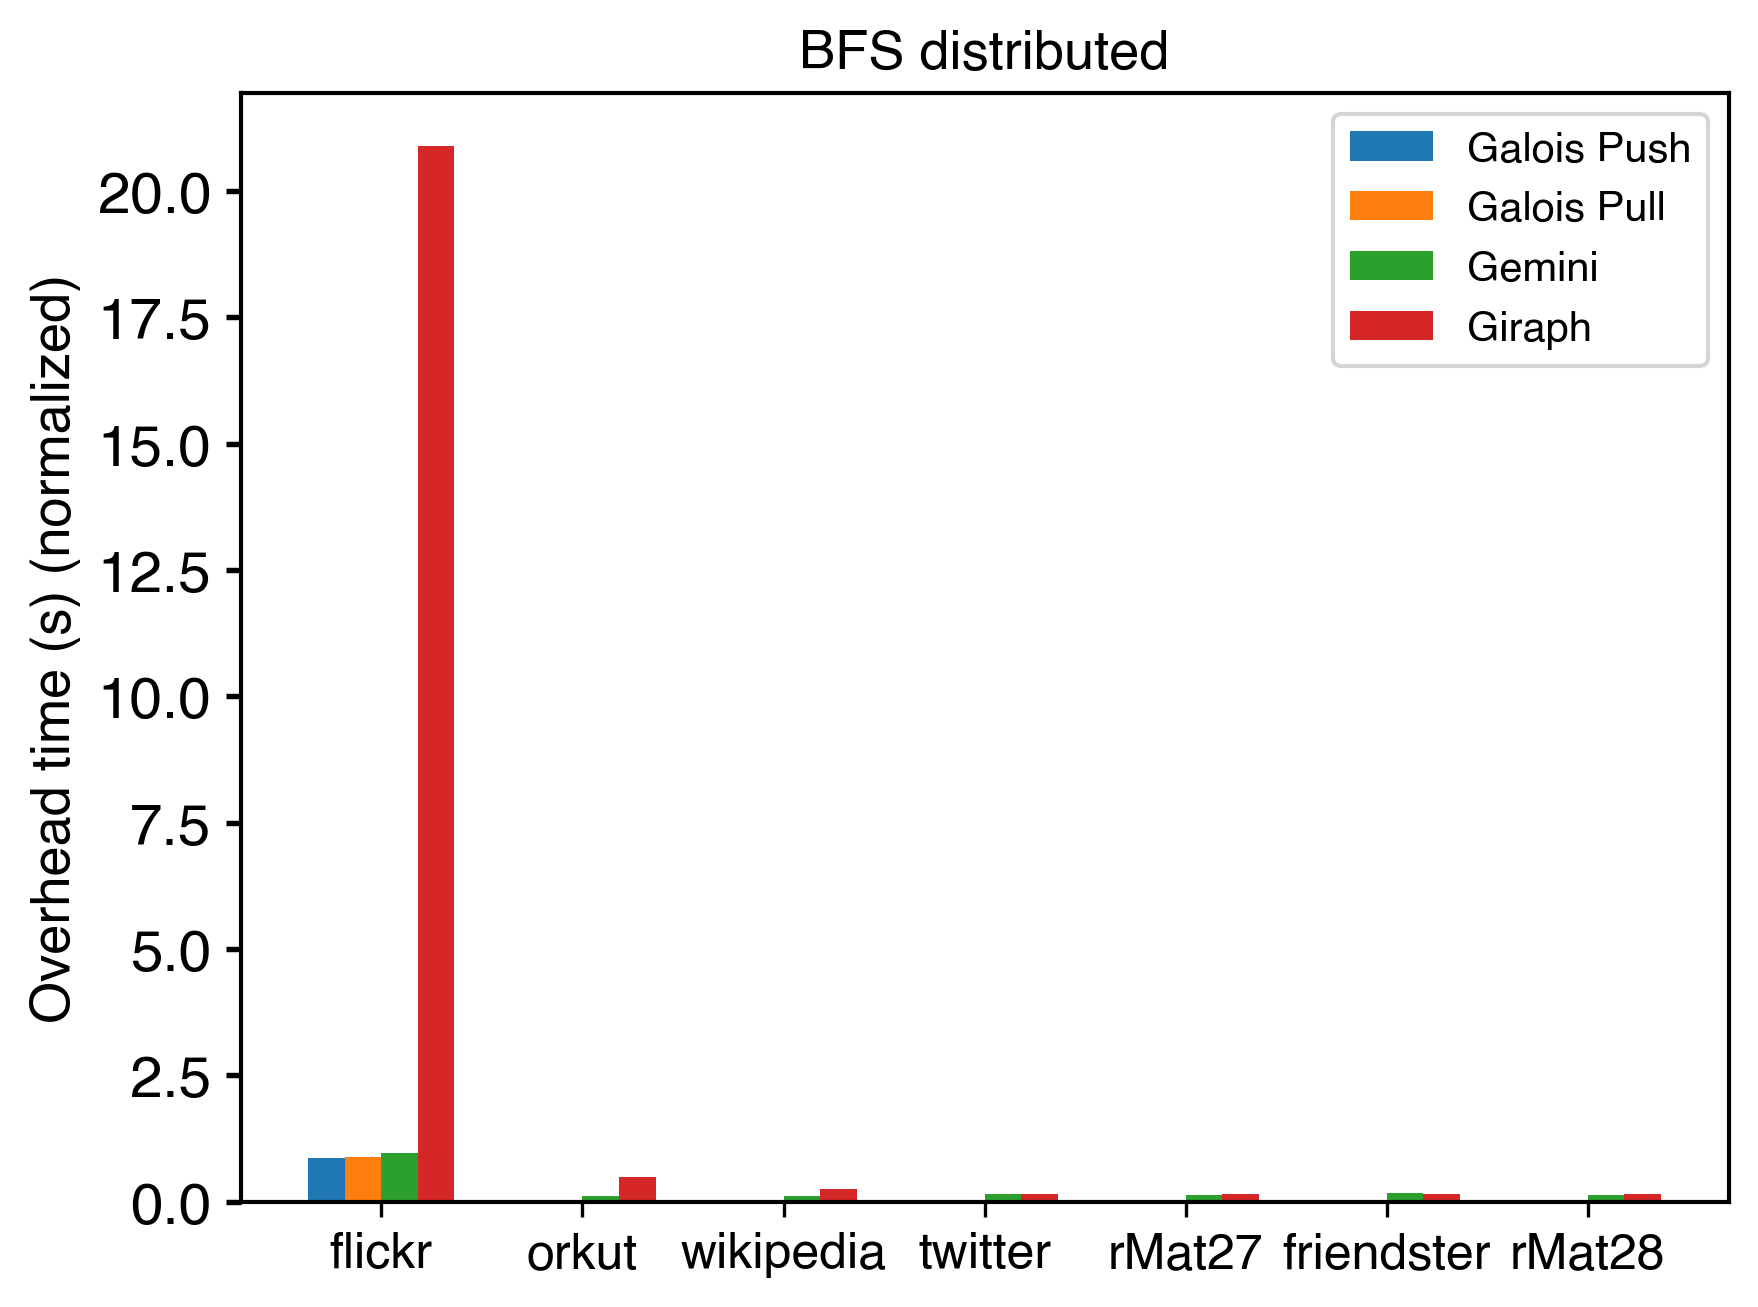
\includegraphics[width=\linewidth]{../../plots/distributedBFS_overheadTimeNormalized.png}
		\caption{Overhead time normalized by the graph size in million edges}
		\label{fig:distributedBFS_overheadNormalized}
	\end{subfigure}
	
	\caption{Average times on the distributed cluster, black bars represent one standard deviation in our testing}
\end{figure*}
